\documentclass[border=10pt]{standalone}
\usepackage{tikz}
\usetikzlibrary{shapes.geometric, arrows.meta, positioning}
\tikzset{
  red-rounded-rectangle/.style={rectangle, rounded corners, minimum width=3cm, minimum height=1cm,text centered, draw=black, fill=red!30, align=center},
  green-rounded-rectangle/.style={rectangle, rounded corners, minimum width=3cm, minimum height=1cm,text centered, draw=black, fill=green!30, align=center},
  blue-rounded-rectangle/.style={rectangle, rounded corners, minimum width=3cm, minimum height=1cm,text centered, draw=black, fill=blue!30, align=center},
}
\begin{document}
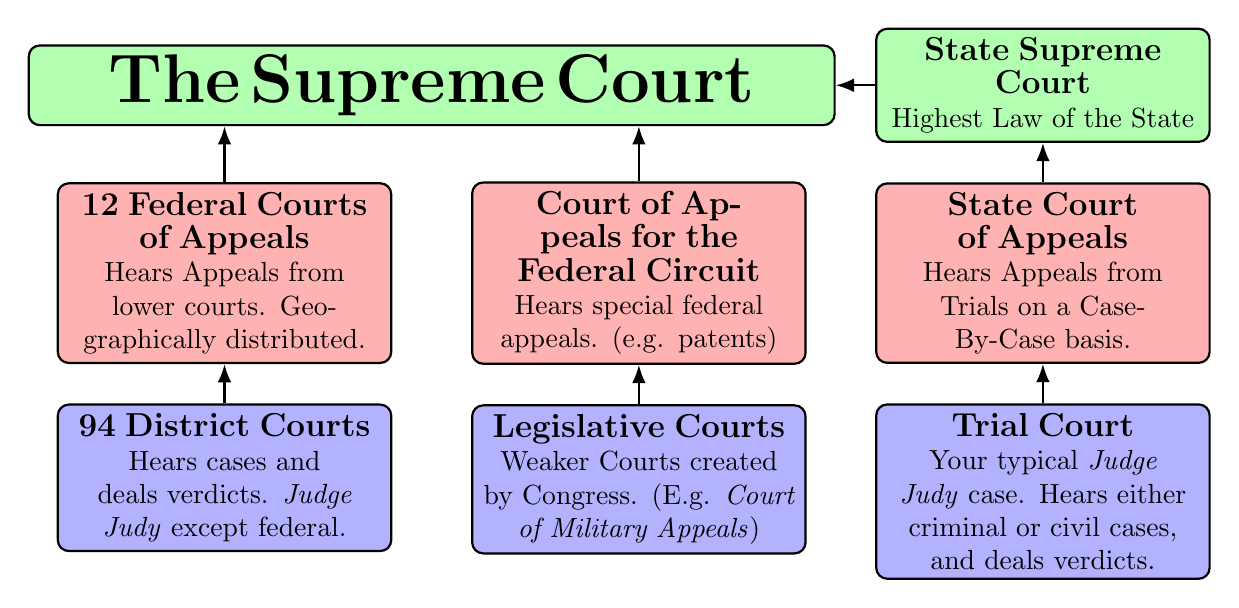
\begin{tikzpicture}[node distance=0.5cm, >/.tip=Latex, thick]
  \node (scotus) [green-rounded-rectangle, text width = 10cm]{
    {\Huge \textbf{The Supreme Court}}
  };
  \node (state) [green-rounded-rectangle, right = of scotus, text width=4cm]{
    {\large \textbf{State Supreme Court}}\\
    Highest Law of the State
  };
  \node (state-appeals) [red-rounded-rectangle, below  = of  state, text width = 4cm]{
    {\large \textbf{State Court of Appeals}}\\
    Hears Appeals from Trials on a Case-By-Case basis.
  };
  \node (12-appeals) [red-rounded-rectangle, left=of state-appeals -| scotus, text width = 4cm] {
    {\large \textbf{12 Federal Courts of Appeals}}\\
    Hears Appeals from lower courts. Geographically distributed.
  };
  \node (94-district) [blue-rounded-rectangle, below = of 12-appeals,, text width=4cm]{
    {\large \textbf{94 District Courts}}\\
    Hears cases and deals verdicts. \textit{Judge Judy} except federal.
  };
  \node (court-appeals) [red-rounded-rectangle, right = of scotus |- state-appeals, text width=4cm]{
    {\large \textbf{Court of Appeals for the Federal Circuit}}\\
    Hears special federal appeals. (e.g. patents)
  };
  \node (legis-courts) [blue-rounded-rectangle, below= of court-appeals, text width = 4cm]{
    {\large \textbf{Legislative Courts}}\\
    Weaker Courts created by Congress. (E.g. \textit{Court of Military Appeals})
  };
  \node (trial-court) [blue-rounded-rectangle, below = of state-appeals,  text width=4cm]{
    {\large \textbf{Trial Court}}\\
    Your typical \textit{Judge Judy} case. Hears either criminal or civil cases, and deals verdicts.
  };
  \draw [->] 
    (trial-court) 	edge (state-appeals) 
    (state-appeals) edge (state) 
    (state) edge (scotus) 
    (legis-courts) edge (court-appeals) 
    (court-appeals) edge (scotus.south -| court-appeals) 
    (94-district) 	edge (12-appeals) 
    (12-appeals) -- 
    (12-appeals |- scotus.south) ;
\end{tikzpicture}
\end{document}  